\documentclass[
  bibliography=totoc,     % Literatur im Inhaltsverzeichnis
  captions=tableheading,  % Tabellenüberschriften
  titlepage=firstiscover, % Titelseite ist Deckblatt
  parskip=half,           % schöner Zeilenabstand
]{scrartcl}

% Paket float verbessern
\usepackage{scrhack}

% Warnung, falls nochmal kompiliert werden muss
\usepackage[aux]{rerunfilecheck}

% unverzichtbare Mathe-Befehle
\usepackage{amsmath}
% viele Mathe-Symbole
\usepackage{amssymb}
% Erweiterungen für amsmath
\usepackage{mathtools}

% Fonteinstellungen
\usepackage{fontspec}
% Latin Modern Fonts werden automatisch geladen
% Alternativ zum Beispiel:
%\setromanfont{Libertinus Serif}
%\setsansfont{Libertinus Sans}
%\setmonofont{Libertinus Mono}

% Wenn man andere Schriftarten gesetzt hat,
% sollte man das Seiten-Layout neu berechnen lassen
\recalctypearea{}

% deutsche Spracheinstellungen
\usepackage{polyglossia}
\setmainlanguage{german}


\usepackage[
  math-style=ISO,    % ┐
  bold-style=ISO,    % │
  sans-style=italic, % │ ISO-Standard folgen
  nabla=upright,     % │
  partial=upright,   % ┘
  warnings-off={           % ┐
    mathtools-colon,       % │ unnötige Warnungen ausschalten
    mathtools-overbracket, % │
  },                       % ┘
]{unicode-math}

% traditionelle Fonts für Mathematik
\setmathfont{Latin Modern Math}
% Alternativ zum Beispiel:
%\setmathfont{Libertinus Math}

\setmathfont{XITS Math}[range={scr, bfscr}]
\setmathfont{XITS Math}[range={cal, bfcal}, StylisticSet=1]

% Zahlen und Einheiten
\usepackage[
  locale=DE,                   % deutsche Einstellungen
  separate-uncertainty=true,   % immer Fehler mit \pm
  per-mode=symbol-or-fraction, % / in inline math, fraction in display math
]{siunitx}

% chemische Formeln
\usepackage[
  version=4,
  math-greek=default, % ┐ mit unicode-math zusammenarbeiten
  text-greek=default, % ┘
]{mhchem}

% richtige Anführungszeichen
\usepackage[autostyle]{csquotes}

% schöne Brüche im Text
\usepackage{xfrac}

% Standardplatzierung für Floats einstellen
\usepackage{float}
\floatplacement{figure}{htbp}
\floatplacement{table}{htbp}

% Floats innerhalb einer Section halten
\usepackage[
  section, % Floats innerhalb der Section halten
  below,   % unterhalb der Section aber auf der selben Seite ist ok
]{placeins}

% Seite drehen für breite Tabellen: landscape Umgebung
\usepackage{pdflscape}

% Captions schöner machen.
\usepackage[
  labelfont=bf,        % Tabelle x: Abbildung y: ist jetzt fett
  font=small,          % Schrift etwas kleiner als Dokument
  width=0.9\textwidth, % maximale Breite einer Caption schmaler
]{caption}
% subfigure, subtable, subref
\usepackage{subcaption}

% Grafiken können eingebunden werden
\usepackage{graphicx}
% größere Variation von Dateinamen möglich
\usepackage{grffile}

% schöne Tabellen
\usepackage{booktabs}

% Verbesserungen am Schriftbild
\usepackage{microtype}

% Literaturverzeichnis
\usepackage[
  backend=biber,
]{biblatex}
% Quellendatenbank
\addbibresource{lit.bib}
\addbibresource{programme.bib}

% Hyperlinks im Dokument
\usepackage[
  unicode,        % Unicode in PDF-Attributen erlauben
  pdfusetitle,    % Titel, Autoren und Datum als PDF-Attribute
  pdfcreator={},  % ┐ PDF-Attribute säubern
  pdfproducer={}, % ┘
]{hyperref}
% erweiterte Bookmarks im PDF
\usepackage{bookmark}

% Trennung von Wörtern mit Strichen
\usepackage[shortcuts]{extdash}

\author{%
  Jan Lukas Schubert\\%
  \href{mailto:jan-lukas.schubert@tu-dortmund.de}{jan-lukas.schubert@tu-dortmund.de}%
  \texorpdfstring{\and}{,}%
  Jan Lukas Späh\\%
  \href{mailto:janlukas.spaeh@tu-dortmund.de}{janlukas.spaeh@tu-dortmund.de}%
}
\publishers{TU Dortmund – Fakultät Physik}


\subject{V46}
\title{Faradayeffekt an Halbleitern}
\date{
  Durchführung: 08.07.19
  \hspace{3em}
  Abgabe: 12.07.19
}

\begin{document}

\maketitle
\thispagestyle{empty}
\tableofcontents
\newpage

\section{Ziel}
\label{sec:Ziel}

Ziel dieses Versuchs ist es elektromagnetische Wellen im Bereich der Mikrowellen
auf Hohlleitern zu Untersuchen. Dafür werden verschiedene Moden bestimmt und
vermessen. Außerdem wird die Frequenz auf zwei verschiedene Arten bestimmt und
die Wellenlänge im Hohlleiter mit der Wellenlänge im freien Raum verglichen. Zudem
wird die Dämpfung des Dämpfungsgliedes vermessen. Zum Schluss wird noch das
Stehwellenverhältnis im Hohlleiter auf drei verschiedene Arten bestimmt.

\section{Theorie}
\label{sec:Theorie}

Laserstrahlen sind elektromagnetische Wellen, die sich von üblichen Lichtquellen durch eine viel höhere Intensität mit fast monochromatischem Licht und einer großen Kohärenzlänge unterscheidet.\\
Sie werden in einer Laserapparatur, die aus drei Hauptbestandteilen zusammengesetzt ist, erzeugt. Ein aktives und ein Pumpmedium erzeugen den Strahl, der von zwei Spiegeln, die den Resonator bilden, zum einen total und zum anderen teilreflektiert wird. Das  ermöglicht eine hohe Verstärkung. Die Medien können in allen klassichen Aggregatzuständen vorliegen, wobei in diesem Versuch ein Laser mit gasförmigen Medien betrachtet wird. Der Aufbau ist schematisch für einen Laser mit Helium als Pump- und Neon als aktivem Medium (He-Ne-Laser) in Abbildung \ref{fig:skizzeLaser} dargestellt.

\begin{figure}
  \centering
  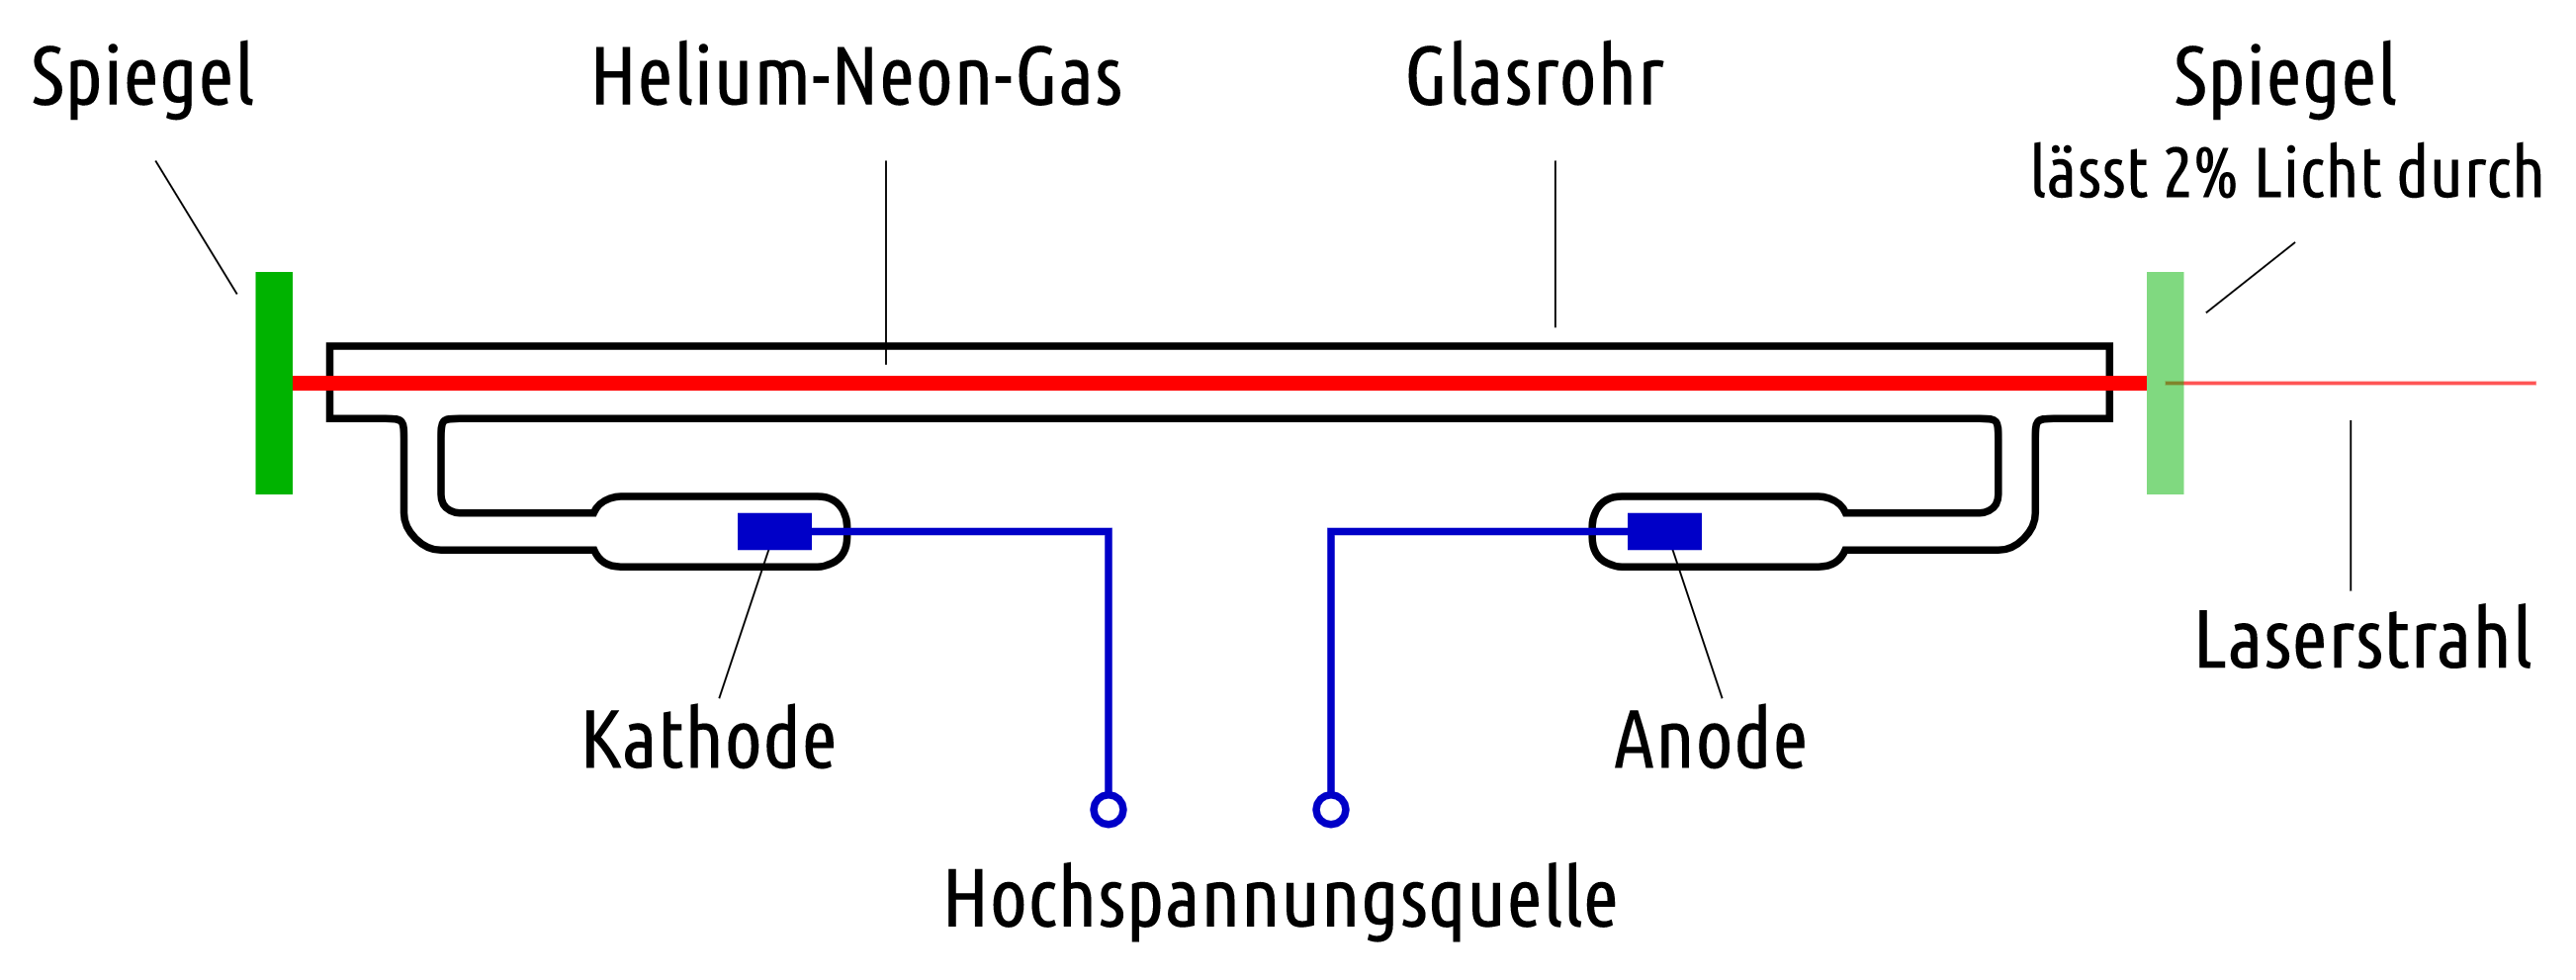
\includegraphics[width=\textwidth]{data/apparatur.png}
  \caption{Darstellung einer Laserappatur für Helium und Neon als Medien.\cite{leifi}}
  \label{fig:skizzeLaser}
\end{figure}

\subsection{Erzeugung von Laserlicht}
\label{sec:erzeugung}
Die Vorgänge bei der Erzeugung von Laserlicht basieren auf drei Wechselwirkungen von Photonen, also elektromagnetischer Strahlung, und den Elektronen in Atomen, die auf diskrete Energieniveaus aufgeteilt sind. Die drei Möglichkeiten sind in Abbildung \ref{fig:mechanismenStrahlung} skizziert.

\begin{figure}
  \centering
  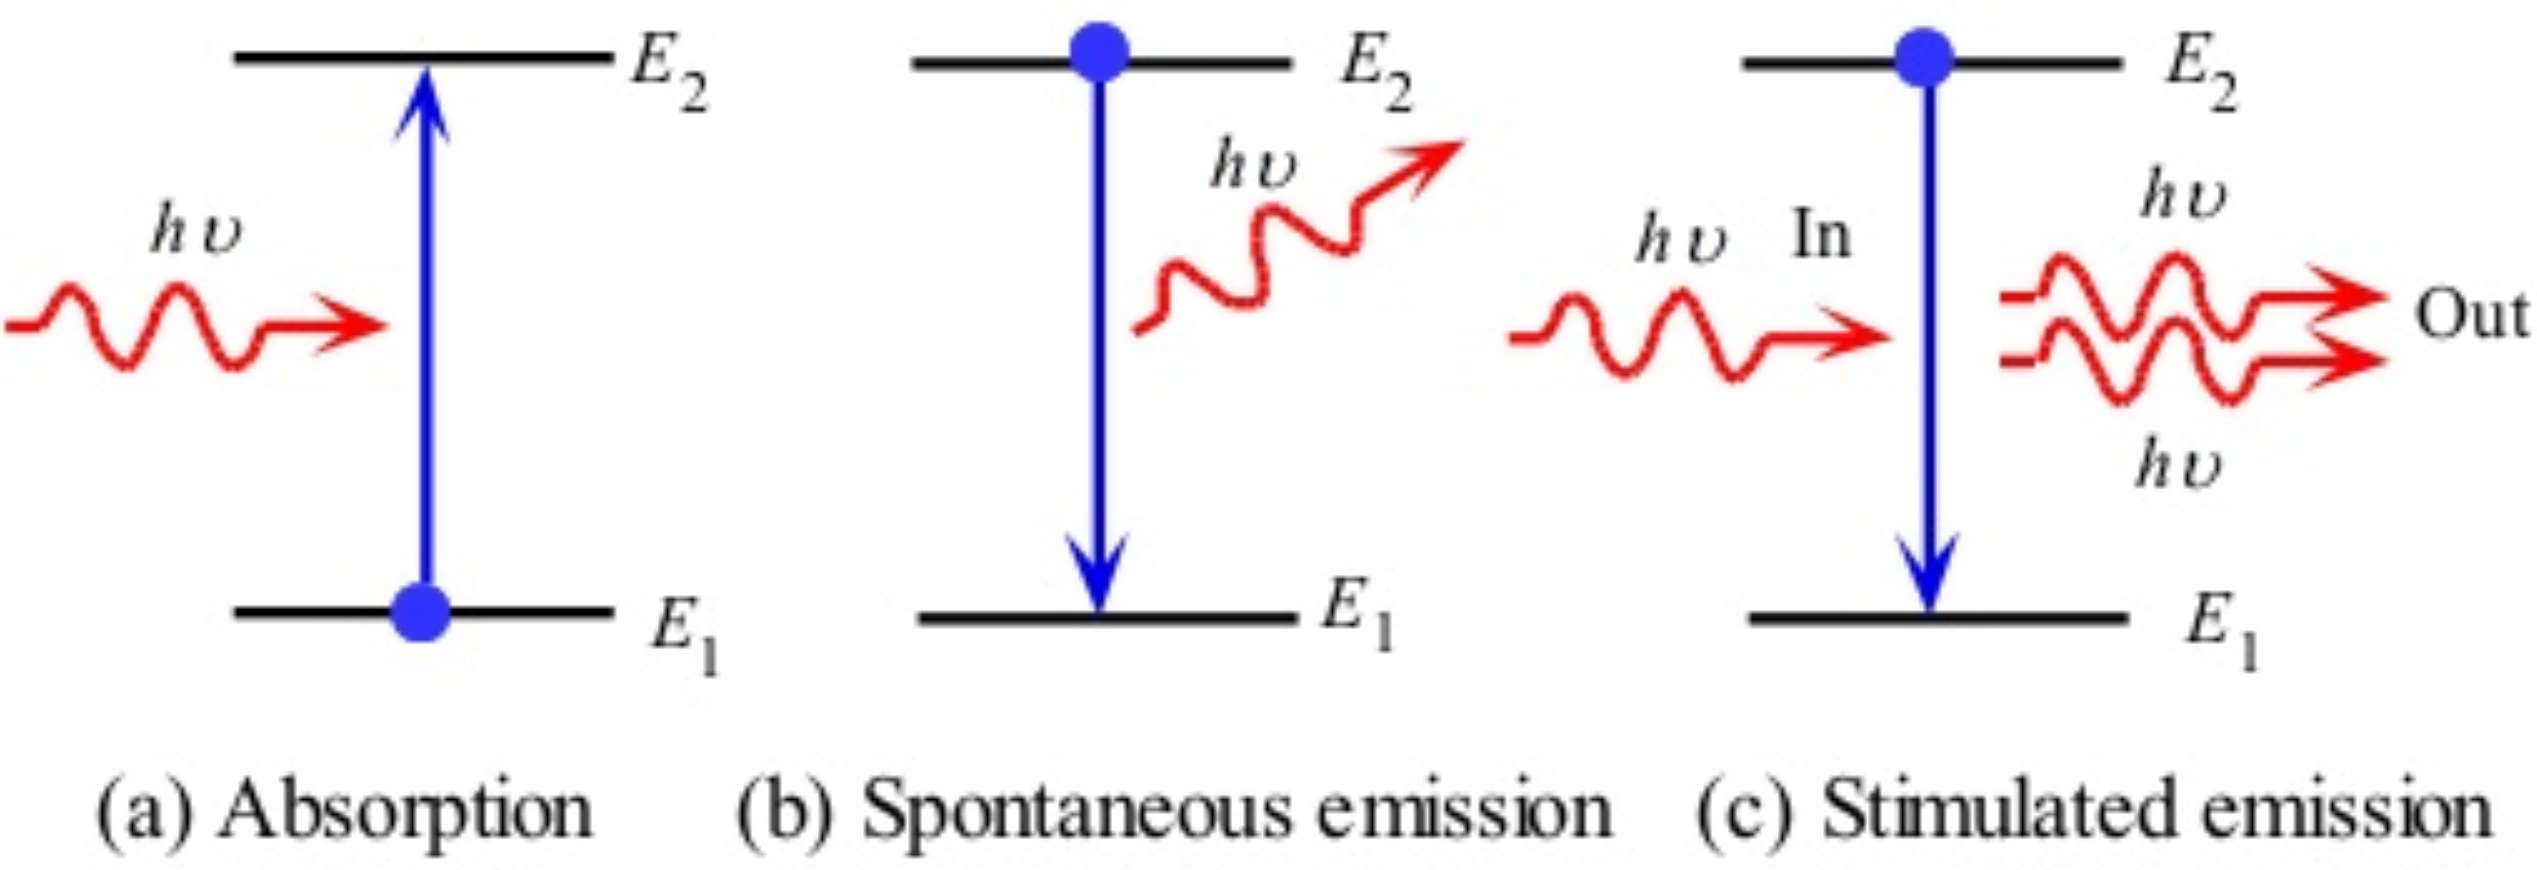
\includegraphics[width=\textwidth]{data/mechanismenStrahlung.png}
  %https://going-postal.com/2017/11/how-does-a-laser-work/pic-01-2/
  \caption{Darstellung der drei fundamentalen Strahlungs-Materie-Wechselwirkungen für die Erzeugung von Laserlicht.\cite{goingPostal}}
  \label{fig:mechanismenStrahlung}
\end{figure}

Bei der Absorption wird ein Photon von einem Atom absorbiert. Dadurch wird ein Elektron von einem niederenergetischen Niveau auf ein höheres Niveau angehoben, seine Energie steigt und das Photon verschwindet. Dieser Prozess kann nur dann stattfinden, wenn das Photon ungefähr eine Energie hat, die der Energiedifferenz der Niveaus entspricht.\\
Die spontane Emission beschreibt das typische Zerfallen von angeregten Zustanden mit einer begrenzten Lebensdauer in Zustände, für die der Übergang erlaubt ist. Dabei wird ein Photon mit zufälliger Phase und Richtung ausgesandt. Seine Energie ist die Energiedifferenz zwischen den beiden Niveaus.\\
Bei der stimulierten Emission löst ein Photon mit der Energie der Energieniveaudifferenz den Zerfall aus. Dabei wird ein weiteres Photon ausgesandt, das dem einfallenden in Richtung, Energie und Phase gleicht. Die beiden Photonen sind somit kohärent.

Es ist ersichtlich, dass nur der Mechanismus der stimulierten Emission eine Möglichkeit bietet, Licht stark zu verstärken, um einen kohärenten, möglichst monochromatischen und nicht zerlaufenden Strahl zu erhalten. Dazu ist eine sogenannte Besetzungsinversion nötig. Die liegt dann vor, wenn ein Niveau oberhalb des Grundzustandes mehr als zur Hälfte gefüllt ist, wobei alle Atome im aktiven Medium betrachtet werden. Dies kann nie in einem Zweiniveausystem geschehen, weil dort die Energie für die Anregung gleich der Energie für die stimulierte Emission ist und diese Prozesse deswegen konkurrieren. Für einen funktionierenden Laser ist somit mindestens ein Dreiniveausystem nötig.\\
Dabei werden Elektronen aus dem Grundzustand in einen hoch angeregten Zustand gehoben. Dies geschieht beim He-Ne-Laser durch Stöße zweiter Art zwischen den Helium- und Neonatomen. Der Zustand zerfällt schnell in einen niedrigeren metastabilen Zustand mit (im Vergleich zum Mutterzustand) hoher Lebensdauer durch spontane Emission. Nun können Photonen mit der passenden Energie die stimulierte Emission hervorrufen und sich somit vervielfältigen. Anfängliche Photonen für diesen Prozess können zum Beispiel aus der spontanen Emission des metastabilen Zustands stammen.

Die Resonatorspiegel sind dafür verantwortlich, die Photonen aus der stimulierten Emission häufig genug erneut durch das aktive Medium gehen zu lassen, um eine Basis für die Besetzungsinversion zu haben. Nur ein geringer Teil der Photonen aus einem Durchlauf durch die Apparatur verlässt als scharfer Laserstrahl den Aufbau.

\subsection{Stabilität des Resonators}
\label{subsec:stabilitaetTheorie}
Für den Stabilitätsparameter $g_1 g_2$ des Resonators muss die Bedingung
\begin{equation}
  0 \le g_1 g_2 \le 1
  \label{eqn:stabilitaet}
\end{equation}
gelten, damit der Resonator optisch stabil ist. Dabei bezeichnet $g_i = 1 - \frac{L}{r_i}$ den Spiegelparameter. Der Abstand der Resonatorspiegel ist $L$ und der Krümmungsradius des Spiegels ist $r_i$.\\
Bei einem optisch stabilen Resonator sind die Verluste kleiner als die Verstärkung durch die stimulierte Emission. Bei konkaven Spiegeln kann insbesondere ein Zusammenfallen der Brennpunkte erreicht werden.

\subsection{Lasermoden}
\label{subsec:modenTheorie}
Die Resonatorlänge $L$ ist viel größer als die Wellenlänge $\lambda$. Damit gibt es viele mögliche Moden. Die Anzahl der Wellenlängen des Lasers im Resonator wird mit q bezeichnet und als Ordnung der longitudinale Mode angesehen. Die Anzahl der Knoten in $x$- und $y$-Richtung werden $l$ und $p$ genannt. Die Eigenschwingungen werden als TEM$_\mathrm{lpq}$ bezeichnet, wobei das $q$ häufig weggelassen wird, weil es für die Untersuchung transversaler Moden nicht von Bedeutung ist. Die radialsymmetrische gaußförmige Grundmode TEM$_{\mathrm{0,0}}$ hat häufig den größten Anteil am Modenspektrum, da diese weniger Verluste als höhere Moden aufweist.

\section{Durchführung}
\label{sec:Durchführung}

\subsection{Aufbau}
\label{subsec:aufbau}

Zur Erzeugung der Mikrowellen wird ein Reflexklystron verwendet. Auf dem Hohhleiter
sind ein Isolator, ein Frequenzmesser und ein Dämpfunglied befestigt. Dies ist
in Abbildung \ref{fig:aufbau} dargestellt. Je nach
Aufgabenteil werden noch ein Stehwellendetektor, ein Abschluss, ein Kurzschluss
und ein Gleitschraubentransformator hinzugefügt. Zur Messung stehen ein Oszilloskop
und ein SWR Meter zur Verfügung.
\begin{figure}
  \centering
  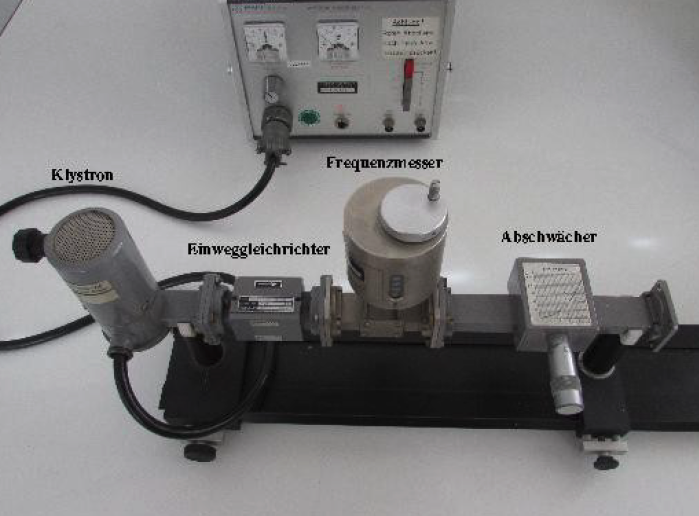
\includegraphics[width=\textwidth]{data/Aufbau.png}
  \caption{Aufbau der zentralen Elemente \cite{Versuchsanleitung_neu}.}
  \label{fig:aufbau}
\end{figure}


\subsection{Untersuchung der Moden}
\label{subsec:moden}
Zur Untersuchung der Moden wird der Versuch gemäß Abbildung \ref{fig:aufbau_mode}
aufgebaut.

\begin{figure}
  \centering
  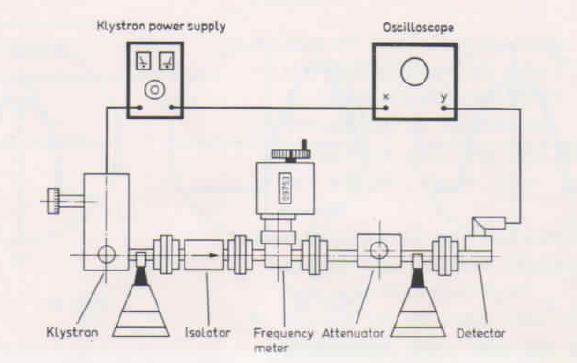
\includegraphics[width=\textwidth]{data/aufbau_mode.png}
  \caption{Aufbau zum Vermessen der Moden \cite{Versuchsanleitung_alt}.}
  \label{fig:aufbau_mode}
\end{figure}

Das Dämpfungsglied wird auf \SI{32}{\decibel} eingestellt und das Signal
wird mit \SI{50}{\hertz} Sinusspannung moduliert. Das Oszilloskop
wird im xy-Modus verwendet. Dabei wird für die x-Achse der Ausgang des Netzgerätes
genutzt und auf der y-Achse die am Ende des Hohlleiters abgegriffene Spannung
verwendet. Anschließend werden Moden sichtbar gemacht. Diese haben einen
Verlauf wie er in Abbildung \ref{fig:mode} dargestellt ist.

\begin{figure}
  \centering
  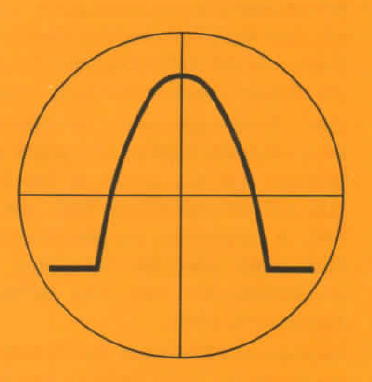
\includegraphics[width=100pt]{data/mode.png}
  \caption{Typischer Verlauf einer Mode \cite{Versuchsanleitung_alt}.}
  \label{fig:mode}
\end{figure}

Mithilfe von Cursorn werden die Startposition des Anstiegs bzw. die Endposition
des Abfalls der Flanken (siehe Abbildung \ref{fig:seite}), sowie die Position des
Maximums und dessen Amplitude bestimmt. Die Daten für die Amplitude werden vom
Oszilloskop abgelesen. Die Werte für die Anstiege und das Maximum werden durch
Variation der Reflektorspannung mit einem Cursor als Fixpunkt bestimmt. Die Reflektorspannung,
bei der sich die Kurve so verschoben hat, dass der zu messende Punkt gerade auf dem
Cursor liegt, wird als Messwert notiert.

\begin{figure}
  \centering
  
\includegraphics[width=100pt]{data/seite.png}
  \caption{Skizze zum Vermessen der Mode mithilfe von Cursorn \cite{Versuchsanleitung_alt}.}
  \label{fig:seite}
\end{figure}

Mithilfe des Frequenzmessers
wird die Frequenz gemessen, indem die Frequenz so lange variiert wird, bis ein
sogenannter dip auf einem der Maxima der Moden liegt (siehe Abbildung \ref{fig:dip}.

\begin{figure}
  \centering
  
\includegraphics[width=100pt]{data/dip.png}
  \caption{Skizze zum Messen der Frequenz mithilfe des Frequenzmessers \cite{Versuchsanleitung_alt}.}
  \label{fig:dip}
\end{figure}

Diese Frequenz entspricht dann der Frequenz der jeweiligen Mode.

\subsection{Bestimmung der Wellenlänge und Frequenz}
\label{subsec:frequenz}
Der Versuch wird gemäß Abbildung \ref{fig:aufbau_frequenz} Umgebaut. Das Dämpfungsglied
wird auf 20dB und die Reflektorspannung auf \SI{163}{\volt} geregelt. Zudem wird das
Signal mit einer \SI{1}{\kilo\hertz} Rechteckspannung moduliert. Anschließend wird
mithilfe des Frequenzmessers die Frequenz gemessen. Anschließend werden mithilfe des
Stehwellendetektors Minima gesucht und deren Positionen notiert.

\begin{figure}
  \centering
  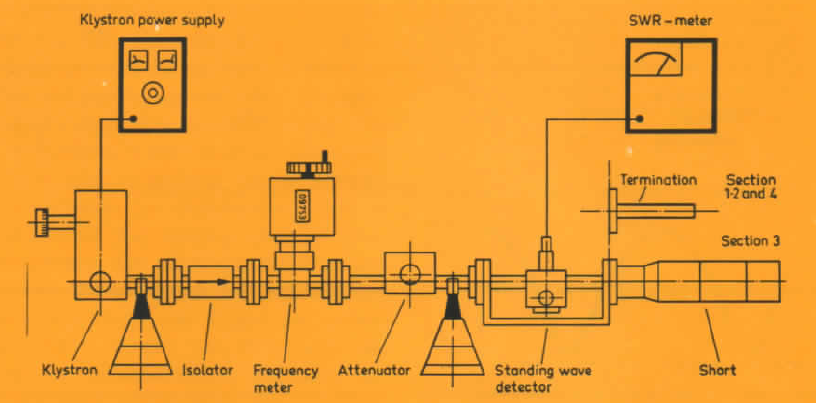
\includegraphics[width=\textwidth]{data/aufbau_frequenz.png}
  \caption{Aufbau zur Wellenlängen- und Frequenzmessung \cite{Versuchsanleitung_alt}.}
  \label{fig:aufbau_frequenz}
\end{figure}

Für einen rechteckigen Hohlleiter ergibt sich für die Frequez im freien Raum
\begin{equation}
  f=c \sqrt{\left(\frac{1}{\lambda_{\symup{g}}}\right)^2+\left(\frac{1}{2a}\right)^2} \,.
\end{equation}

\subsection{Bestimmung der Dämpfung des Mikrowellenfeldes}
\label{subsec:dämpfung}
Bei gleichem Aufbau wird die Dämpfung von 0 aus immer weiter aufgedreht. Bei jedem
vollen Dezibelschritt auf dem SWR Meter wird der Stand der Mikrometerschraube
abgelesen und das Wertepaar notiert.


\subsection{Bestimmung des Stehwellenverhältnisses}
\label{subsec:swr}

Das Stehwellenverhältnis wird über drei verschiedene Verfahren bestimmt: Die direkte
Methode, die für kleine und mittlere SWR geeignet ist, die 3dB Methode, die für hohe
SWR verwendet wird und die Abschwächer Methode, die ebenfalls für hohe SWR verwendet
wird. Es wird der Aufbau aus Abbildung \ref{aufbau_swr} verwendet.

\begin{figure}
  \centering
  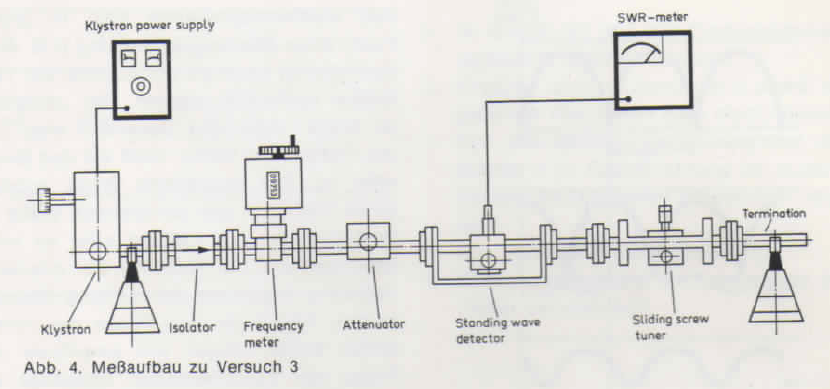
\includegraphics[width=\textwidth]{data/aufbau_swr.png}
  \caption{Aufbau zur Messung des Stehwellenverhältnisses \cite{Versuchsanleitung_alt}.}
  \label{fig:aufbau_swr}
\end{figure}

Bei der
direkten Methode wird die Sonde auf der Leitung in ein Maximum verschoben. Dieser
Wert wird dann auf dem SWR Meter mittels der Verstärkung auf 1 geregelt. Danach
wird mit der Sonde ein Minimum gesucht und der zugehörige Wert vom SWR Meter
abgelesen. Dieses Verfahren wird für Stifttiefen von 0, 3, 5, 7, und \SI{9}{\milli\meter}
durchgeführt.

Bei der 3dB Methode wird die Sonde bei \SI{9}{\milli\meter} Stifttiefe in ein
Minimum gefahren. Daraufhin wird mittels Verstärkung der Zeiger des SWR Meters auf
3dB auf der unteren Skala geregelt. Dann werden links und rechts von dem Minimum
Stellen gesucht, an denen sich ein Vollausschlag einstellt. Die Schlittenpositionen
dieser beiden Stellen werden notiert. Es lässt sich über den Zusammenhang
\begin{equation}
  S=\sqrt{1+\frac{1}{\sin^2\left(\frac{\pi(x_1-x_2)}{\lambda_{\symup{g}}}\right)}}
  \label{3dB}
\end{equation}
das Stehwellenverhältnis bestimmen. Dabei sind $x_{\symup{i}}$ die beiden gemessenen
Schlittenpositionen.

Für die Abschwächermethode wird die Sonde bei \SI{9}{\milli\meter} Stifttiefe in ein
Minimum gefahren und das Dämpfungsglied auf \SI{20}{\decibel} eingestellt. Dann
weren gleichzeitig die Sonde verschoben und die Dämpfung erhöht, sodass sich im
Maximum die gleiche Zeigerposition wie zuvor im Minimum ergibt. Daraus kann dann
das Stehwellenverhältnis mit Hilfe von
\begin{equation}
  S=10^{\frac{A_2-A_1}{20}}
  \label{abschwaecher}
\end{equation}
berechnet werden. Hier sind $A_{\symup{i}}$ die eingestellten Dämpfungen.

%\section{Fehlerrechnung}
\label{sec:Fehlerrechnung}
Der Mittelwert einer Stichprobe von $N$ Werten wird durch
\begin{equation}
  \overline{x} = \sum\limits_{i = 1}^N x_i
  \label{eqn:mean}
\end{equation}

berechnet.
Die empirische Standardabweichung dieser Stichprobe ist durch
\begin{equation}
  \sigma_x = \sqrt{\frac{1}{N-1}
    \sum\limits_{i = 1}^N
    (x_i-\overline{x})^2}
    \label{eqn:std}
\end{equation}

gegeben.
Ist $f$ eine Funktion, die von unsicheren Variablen $x_i$ mit
Standardabweichungen $\sigma_i$ abhängt, so ist die Unsicherheit von f
\begin{equation}
  \sigma_f = \sqrt{
    \sum\limits_{i = 1}^N
      \left( \frac{\partial f}{\partial x_i} \sigma_i \right)^{\!\! 2}
  }\,.
  \label{eqn:gaussfehler}
\end{equation}

Diese Formel bezeichnet man als "Gauß'sches Fehlerfortpflanzungsgesetz".

Bei einer linearen Regression folgt eine Ausgleichsgerade
\begin{equation}
  y(x) = ax+b\,
\end{equation}
mit der Steigung $a$ und dem Ordinatenabschnitt $b$. Liegen Fehler in y-Richtung
und nur in y-Richtung vor, dann sind die Parameter $a$ und $b$ selbst unsicher
und ergeben sich zu
\begin{align}
  a &= \frac{\overline{xy}-\overline{x} \cdot \overline{y}}{\overline{x^2}-\overline{x}^2}\,,\\
  b &= \frac{\overline{y}-\overline{x^2}-\overline{xy} \cdot \overline{x}}{\overline{x^2}-\overline{x}^2}\,.
\end{align}

%Wenn im Folgenden Mittelwerte, Standardabweichungen und Fehler von
%Funktionen unsicherer Größen berechnet werden, so werden stets die obigen
%Formeln verwendet.
Jegliche Rechnungen werden mit IPython 5.3.0 in Python 3.6.1 durchgeführt. Dabei
werden die Bibliotheken "numpy" \cite{numpy} und "scipy" \cite{scipy} verwendet.
Letztere dient insbesondere zur Erstellung von Ausgleichsrechnungen.
Die Ausführung von Fehlerrechnungen geschieht unter Verwendung des Pakets
"uncertainties" \cite{uncertainties}. Zur Erstellung von Graphen wird die Bibliothek
"matplotlib" \cite{matplotlib} verwendet.

\section{Auswertung}
\label{sec:Auswertung}

\subsection{Überprüfung der Stabilität}
\label{subsec:stabilitaet}
Die Messwerte für den realisierten Laser mit einem flachen und einem sphärischen
Spiegel befinden sich in Tabelle \ref{tab:plankonkav}. In Abbildung \ref{fig:plankonkav}
sind die gemessenen Stromstärken $I$ gegen die Resonatorlängen $L$ aufgetragen.
Zudem wird eine lineare Ausgleichrechung der Form
\begin{equation*}
  f(L)=a L+b
\end{equation*}
durchgeführt. Für die Berechnungen wird Python 3.7.1, unterstützt von dem Paket
NumPy \cite{numpy} genutzt. Für die Grafiken
wird die Python Bibliothek matblotlib \cite{matplotlib} verwendet.
Die Ausgleichsrechnungen werden mithilfe von SciPy \cite{scipy} durchgeführt.
Für die Parameter $a$ und $b$ ergeben sich die Werte
\begin{align*}
  a&= \SI{2.61(029)}{\micro\ampere\per\centi\per\metre}\,,\\
  b&= \SI{214(18)}{\micro\ampere}\,.
\end{align*}

\begin{figure}
  \centering
  \includegraphics{build/plankonkav.pdf}
  \caption{Darstellung der Messwerte sowie der Ausgleichsfunktion für den
  Resonator aus einem flachen und einem sphärischen Spiegel.}
  \label{fig:plankonkav}
\end{figure}

Die Messwerte für den Resonator aus zwei sphärischen Spiegeln befinden sich in
Tabelle \ref{tab:konkavkonkav}. In Abbildung \ref{fig:konkavkonkav} sind die gemessenen Stromstärken gegen die Resonatorlänge aufgetragen. Außerdem wird eine
Ausgleichsfunktion der Form
\begin{equation*}
  f(L)=a L^2 + b L + c
\end{equation*}
angesetzt. Es ergeben sich die Parameter
\begin{align*}
  a&= \SI{0.097(017)}{\micro\ampere\per\centi\per\metre\squared}\,, \\
  b&= \SI{-21(4)}{\micro\ampere\per\centi\per\metre}\,, \\
  c&= \SI{1.15(020)e3}{\micro\ampere}\,.
\end{align*}

\begin{figure}
  \centering
  \includegraphics{build/konkavkonkav.pdf}
  \caption{Darstellung der Messwerte sowie der Ausgleichsfunktion für den
  Resonator aus zwei sphärischen Spiegeln.}
  \label{fig:konkavkonkav}
\end{figure}

\subsection{Vermessung der Moden}
\label{subsec:moden}

Die gemessenen Werte für die TEM$_{\mathrm{00}}$ Mode befinden sich in den Tabellen \ref{tab:tem00a} und \ref{tab:tem00b}. In Abbildung \ref{fig:tem00} sind sie
grafisch dargestellt. Die Werte zeigen nicht den theoretisch zu erwartenden gaußförmigen
Verlauf. In Abbildung \ref{fig:bild} ist ein Bild dieser Mode eingefügt. Auch dort
ist im Zentrum eine geringere Intensität zu erkennen.

Trotz der Abweichungen wird eine Ausgleichsrechnung mit einer gaußförmigen Funktion
\begin{equation*}
  I_{0,0}(L)=I_{\text{max}} \exp\left(-2 \left(\frac{L-d}{\omega}\right)^2\right)
\end{equation*}
durchgeführt. Dabei ist $I_{\text{max}}$ der maximale Strom, $d$ eine Verschiebung in
x-Richtung und $\omega$ der Strahlradius. Es ergeben sich die Parameter
\begin{align*}
  I_{\text{max}}&=\SI{597(29)}{\micro\ampere} \,,\\
  d&= \SI{-3.2(8)}{\milli\metre} \,, \\
  \omega&=\SI{27.8(17)}{\milli\metre} \,.
\end{align*}

\begin{figure}
  \centering
  \includegraphics{build/tem00.pdf}
  \caption{Darstellung der Messwerte sowie der Ausgleichsfunktion für die TEM$_{\mathrm{00}}$ Mode.}
  \label{fig:tem00}
\end{figure}

\begin{figure}
  \centering
  \includegraphics[width=0.7\textwidth]{data/tem00.png}
  \caption{Bild der TEM$_{\mathrm{00}}$ Mode. Deutlich zu erkennen ist eine schwächere Intensität im Zentrum.}
  \label{fig:bild}
\end{figure}


Die Messwerte für die TEM$_{\mathrm{01}}$ Mode sind in den Tabellen \ref{tab:tem01a} und \ref{tab:tem01b} aufgeführt. In Abbildung \ref{fig:tem01} sind sie grafisch dargestellt. Als Ausgleichsfunktion wird ein Produkt von Parabel und Gaußverteilung in der Form
\begin{equation*}
  I_{0,1}=I_{\text{max}}\left(\frac{L-d}{\omega}\right)^2 \exp\left(-2\left(\frac{L-d}{\omega}\right)^2\right)
\end{equation*}
angesetzt.
Die Ausgleichsrechnung liefert die Parameter
\begin{align*}
  I_{\text{max}}&=\SI{1.27(05)e3}{\nano\ampere} \,,\\
  d&=\SI{0.38(28)}{\milli\metre} \,,\\
  w&=\SI{15.0(4)}{\milli\metre} \,.
\end{align*}

\begin{figure}
  \centering
  \includegraphics{build/tem01.pdf}
  \caption{Darstellung der Messwerte sowie der Ausgleichsfunktion für die TEM$_{\mathrm{01}}$ Mode.}
  \label{fig:tem01}
\end{figure}

\subsection{Messung der Polarisierung}
\label{subsec:polarisierung}

In Tabelle \ref{tab:polarisation} befinden sich die Messwerte zur Intensität des
Laserstrahls in Abhängigkeit von dem Winkel des Polarisationsfilters. Diese Werte
sind in Abbildung \ref{fig:polarisation} graphisch dargestellt. Die Ausgleichsfunktion ist
\begin{equation*}
  f(\phi)=I_{\text{max}} \cos^2(\phi+\delta)\,.
\end{equation*}
Die Ausgleichsrechnung liefert die Parameter
\begin{align*}
  I_{\text{max}}&=\SI{56.02(118)}{\micro\ampere} \,, \\
  \delta&=\SI{919.32(105)} \,.
\end{align*}

\begin{figure}
  \centering
  \includegraphics{build/polarisation.pdf}
  \caption{Darstellung der Messwerte sowie der Ausgleichsfunktion für die Intensität in
  Abhängigkeit vom Winkel des Polarisationsfilters.}
  \label{fig:polarisation}
\end{figure}

In der Ausgleichsrechnung ist eine Phasenverschiebung von etwa -20° ersichtlich.

\subsection{Bestimmung der Wellenlänge}
\label{subsec:wellenlaenge}
Zur Bestimmung der Wellenlänge des Lasers wurden die Werte
\begin{align*}
  d_1&=\SI{6.3(2)}{\centi\metre} \,,\\
  d_2&=\SI{6.2(2)}{\centi\metre}  \,,\\
  l&=\SI{95.7(2)}{\centi\metre} \,.
\end{align*}
gemessen.
Die beiden Messwerte für $d$ werden gemittelt und es ergibt sich $\SI{6.25(14)}{\centi\metre}$
\footnote{Ist $f$ eine Funktion, die von unsicheren Variablen $x_i$ mit
Standardabweichungen $\sigma_i$ abhängt, so ist die Unsicherheit von f gegeben durch
  $\sigma_f = \sqrt{
    \sum\limits_{i = 1}^N
      \left( \frac{\partial f}{\partial x_i} \sigma_i \right)^{\!\! 2}
  }\,.$
}
, wobei die Unsicherheit sich zu $\sigma_d = \frac{1}{2} \sqrt{\sigma_{d_1}^2+\sigma_{d_2}^2} = \frac{\sqrt{2}}{10}\,\text{cm}$
bestimmt.
Mithilfe des Zusammenhangs
\begin{equation*}
  \lambda= g \sin \left(\arctan\left(\frac{d}{l}\right)\right)
\end{equation*}
lässt sich daraus die Wellenlänge berechnen. Dabei ist $l$ der Abstand zwischen
Gitter und Schirm, $d$ der Abstand der ersten Hauptmaxima vom nullten Hauptmaximum
auf dem Schirm und g ist die Spaltbreite des Gitters. Das verwendete Gitter hat eine
Spaltbreite von $10^{-5}$\,m. Damit ergibt sich für die Wellenlänge des Lasers der Wert
\begin{align*}
  \lambda=\SI{652(15)}{\nano\metre}\,.
\end{align*}
Die Unsicherheit von $\lambda$ lässt sich mit
\begin{equation}
  \sigma_\lambda = \sqrt{\frac{d^{2} g^{2} \sigma_{l}^{2}}{l^{4} \left(\frac{d^{2}}{l^{2}} + 1\right)^{2}} + \frac{g^{2} \sigma_{d}^{2}}{l^{2} \left(\frac{d^{2}}{l^{2}} + 1\right)^{2}} {\left (\frac{d}{l} \right )}}
\end{equation}
berechnen.
Der theoretisch zu erwartende Wert ist $\lambda= 632,8$\,mm. Der experimentell bestimmte
Wert weicht davon um $3,0$\,\% ab.

\section{Diskussion}
\label{sec:Diskussion}

Der Versuch lässt sich insgesamt nur teilweise als erfolgreich bewerten. Die bestimmte
Schallgeschwindigkeit ist mit $\SI{339.7(7)}{\meter\per\second}$ und einer relativen Abweichung zum Theoriewert
von $-0{,}85\%$ sehr genau.
Der in den Abbildungen \ref{fig:zyl2}, \ref{fig:zyl12} und \ref{fig:zyl1} bis \ref{fig:zyl11}
dargestellte Vergleich zwischen den Messungen am Zylinderresonator mithilfe des Oszilloskops und denen mithilfe des
Computers zeigt jedoch Unstimmigkeiten. Für kurze Resonatoren stimmen die Messwerte recht
gut überein, für große Resonatorlängen sind jedoch starke Abweichungen zu erkennen. Der Grund
dafür liegt vermutlich im falschen Betrieb des Lautsprechers und des Mikrofons. Wegen großer
Probleme bei der Inbetriebnahme dieser Instrumente wurde vermutlich ohne externe Soundkarte
gemessen, sodass Lautsprecher und Mikrofon nicht ordnungsgemäß gearbeitet haben.
Auffällig ist, dass die mit dem Computer gemessenen Werte für die Resonanzfrequenzen
nicht äquidistant sind. Das ist ein Widerspruch zu der linearen Dispersion und weist auf
Messfehler hin.

Für den Kugelresonator hingegen zeigt sich eine sehr gute Übereinstimmung zwischen der Messung
am Oszilloskop und der am Computer (vgl. Abbildung \ref{fig:hatomalles}). Die Messwerte für die
Amplitude in Abhängikeit vom Verschiebungswinkel $\alpha$ des Lautsprechers und des Mikrophons
zeigen nur tendenziell eine Analogie zu den gezeigten Theoriekurven. Die Abweichungen sind
jedoch zu groß um eine Aussage darüber treffen zu können, ob die gemessenen Werte
tatsächlich dem Verlauf dieser Kurve folgen. Möglicherweise sind auch die Funktionen
für die Theoriekurven nicht passend gewählt.

In Bezug auf die Quantenanalogien konnte das diskrete Frequenzspektrum des Zylinderresonators, welches in Analogie zu dem diskreten Energiespektrum des eindimensionalen Potenzialtopfes steht, gemessen werden. Zudem konnte
eine grobe Anordnung der Messwerte auf den Graphen der Legendrepolynome gezeigt werden. Dies zeigt, dass die Kugelfächenfunktionen des Kugelresonators denen des
Wasserstoffatoms entsprechen könnten. Um aussagekräftige Ergebnisse über Quantenanalogien treffen zu können müssten allerdings mehr und insbesondere genauere Messungen durchgeführt werden.

\newpage
\addsec{Anhang}
\label{sec:Anhang}

\begin{table}[htp]
  \caption{Messwerte für den Resonator aus einem flachen und einem gebogenen Spiegel(KRÜMMUNGSRADIUS?!).}
  \label{tab:plankonkav}
	\begin{center}
		\begin{tabular}{cc}
		\toprule
			{$L$/cm} & {$I$/\mu A}\\
			\midrule
			43,2 & 100\\
			45,0 & 100\\
			47,0 & 120\\
			49,5 & 90\\
			51,0 & 90\\
			52,5 & 80\\
			54,0 & 80\\
			55,0 & 60\\
			56,9 & 30\\
			58,3 & 60\\
			60,7 & 50\\
			62,5 & 30\\
			64,7 & 30\\
			67,1 & 30\\
			68,9 & 30\\
			70,7 & 30\\
			72,1 & 25\\
			73,1 & 35\\
			74,6 & 25\\
			76,0 & 35\\
			78,9 & 15\\
		\bottomrule
		\end{tabular}
	\end{center}
\end{table}

\begin{table}[htp]
  \caption{Messwerte für den Resonator aus zwei gebogenen Spiegeln(KRÜMMUNGSRADIUS?!).}
  \label{tab:konkavkonkav}
	\begin{center}
		\begin{tabular}{cc}
		\toprule
			{$L$/cm} & {$I$/\mu A}\\
			\midrule
			71,2 & 180\\
			74,8 & 180\\
			76,5 & 200\\
			78,3 & 160\\
			80,2 & 130\\
			82,8 & 120\\
			84,9 & 130\\
			86,9 & 120\\
			88,5 & 100\\
			90,9 & 60\\
			94,0 & 10\\
			96,4 & 0\\
			97,5 & 70\\
			99,3 & 70\\
			101,7 & 70\\
			105,1 & 30\\
			108,5 & 60\\
			111,3 & 50\\
			112,5 & 140\\
			116,5 & 70\\
			120,6 & 70\\
			124,4 & 140\\
			128,6 & 110\\
			132,7 & 240\\
			136,2 & 240\\
			139,1 & 230\\
			144,2 & 220\\
			147,4 & 170\\
			149,5 & 180\\
		\bottomrule
		\end{tabular}
	\end{center}
\end{table}

\begin{table}[htp]
	\begin{center}
    \caption{Messwerte für die $TEM_{0,0}$ Mode.}
    \label{tab:tem00a}
		\begin{tabular}{cc}
		\toprule
			{$L$/cm} & {$I$/nA}\\
			\midrule
			-31 & 17,7\\
			-20 & 18,5\\
			-29 & 21\\
			-28 & 22\\
			-27 & 28\\
			-26 & 33\\
			-25 & 42\\
			-24 & 55\\
			-23 & 85\\
			-22 & 115\\
			-21 & 150\\
			-20 & 190\\
			-19 & 240\\
			-18 & 315\\
			-17 & 360\\
			-16 & 420\\
			-15 & 550\\
			-14 & 600\\
			-13 & 640\\
			-12 & 680\\
			-11 & 750\\
			-10 & 750\\
			-9 & 750\\
			-8 & 740\\
			-7 & 695\\
			-6 & 660\\
			-5 & 610\\
			-4 & 530\\
			-3 & 490\\
			-2 & 440\\
			-1 & 385\\
			0 & 350\\
			1 & 330\\
			2 & 350\\
			3 & 380\\
			4 & 410\\
			5 & 435\\
			6 & 430\\
			7 & 460\\
			8 & 470\\
			9 & 470\\
			10 & 460\\
		\bottomrule
		\end{tabular}
	\end{center}
\end{table}

\begin{table}[htp]
	\begin{center}
    \caption{Messwerte für die $TEM_{0,0}$ Mode (Fortsetzung).}
    \label{tab:tem00b}
		\begin{tabular}{cc}
		\toprule
			{$L$/cm} & {$I$/nA}\\
			\midrule
      11 & 450\\
      12 & 425\\
      13 & 410\\
      14 & 380\\
      15 & 355\\
      16 & 320\\
      17 & 270\\
      18 & 250\\
      19 & 220\\
      20 & 190\\
      21 & 160\\
      22 & 125\\
      23 & 100\\
      24 & 80\\
      25 & 65\\
      26 & 55\\
      27 & 45\\
      28 & 40\\
      29 & 36\\
      30 & 31\\
      31 & 29\\
      \bottomrule
    \end{tabular}
  \end{center}
\end{table}

\begin{table}[htp]
	\begin{center}
    \caption{Messwerte für die $TEM_{0,1}$ Mode.}
    \label{tab:tem01a}
		\begin{tabular}{cc}
		\toprule
			{$L$/cm} & {$I$/nA}\\
			\midrule
			-31 & 15\\
			-30 & 18\\
			-29 & 19\\
			-28 & 20\\
			-27 & 24\\
			-26 & 27\\
			-25 & 28\\
			-24 & 41\\
			-23 & 52\\
			-22 & 63\\
			-21 & 77\\
			-20 & 95\\
			-19 & 99\\
			-18 & 118\\
			-17 & 70\\
			-16 & 170\\
			-15 & 235\\
			-14 & 255\\
			-13 & 235\\
			-12 & 280\\
			-11 & 299\\
			-10 & 305\\
			-9 & 285\\
			-8 & 265\\
			-7 & 245\\
			-6 & 225\\
			-5 & 120\\
			-4 & 116\\
			-3 & 110\\
			-2 & 65\\
			-1 & 23\\
			0 & 23\\
			1 & 19\\
			2 & 24\\
			3 & 35\\
			4 & 54\\
			5 & 77\\
			6 & 100\\
			7 & 120\\
			8 & 142\\
			9 & 168\\
			10 & 178\\
		\bottomrule
		\end{tabular}
	\end{center}
\end{table}


\begin{table}[htp]
	\begin{center}
    \caption{Messwerte für die $TEM_{0,1}$ Mode (Fortsetzung).}
    \label{tab:tem01b}
		\begin{tabular}{cc}
		\toprule
			{$L$/cm} & {$I$/nA}\\
			\midrule
      11 & 180\\
      12 & 182\\
      13 & 160\\
      14 & 120\\
      15 & 100\\
      16 & 90\\
      17 & 80\\
      18 & 90\\
      19 & 75\\
      20 & 65\\
      21 & 55\\
      22 & 50\\
      23 & 45\\
      24 & 38\\
      25 & 33\\
      26 & 27\\
      27 & 26\\
      28 & 25\\
      29 & 23\\
      30 & 22\\
      31 & 21\\
      \bottomrule
  	\end{tabular}
  \end{center}
\end{table}

\begin{table}[htp]
	\begin{center}
    \caption{Messwerte für die Intensität in Abhängigkeit vom Winkel des Polarisationsfilters.}
    \label{tab:polarisation}
		\begin{tabular}{cc}
		\toprule
			{$\phi$/°} & {$I$/µA}\\
			\midrule
			0 & 45\\
			10 & 37\\
			20 & 34\\
			30 & 28\\
			40 & 18\\
			50 & 9\\
			60 & 2,7\\
			70 & 0,2\\
			80 & 0,95\\
			90 & 5,4\\
			100 & 11\\
			110 & 20\\
			120 & 31\\
			130 & 38\\
			140 & 44\\
			150 & 52\\
			160 & 62\\
			170 & 55\\
			180 & 40\\
			190 & 36\\
			200 & 33\\
			210 & 24\\
			220 & 16\\
			230 & 8,2\\
			240 & 2,7\\
			250 & 0,23\\
			260 & 0,84\\
			270 & 5,6\\
			280 & 13\\
			290 & 22\\
			300 & 32\\
			310 & 41\\
			320 & 51\\
			330 & 68\\
			340 & 67\\
			350 & 53\\
		\bottomrule
		\end{tabular}
	\end{center}
\end{table}

\newpage
\printbibliography

\end{document}
